\chapter{Desarrollo de la Arquitectura de la Información}

\section{Definición de Objetivos del proyecto}
\subsection{Objetivo General}

Crear una aplicación web moderna, fácil de actualizar, compuesta por un Back-End desarrollado en Asp .Net Core y un Front-End, que permita realizar el registro de los participantes y su asistencia a las conferencias.

\subsection{Objetivos Específicos}
 
\begin{itemize}
	\item Desarrollar la arquitectura de la información.
	\item Elaborar una lista de los requerimientos y clasificarlos.
	\item Desarrollar los diagramas UML.
	\item Elaborar el diagrama E-R y Relacional de la base de datos.
\end{itemize}

\section{Definición de Audiencia}
La presente aplicación va dirigida al personal docente del ITL.

\section{Definición de Contenidos del Proyecto}
La aplicación que se realizó consta de las siguientes partes:
\subsection{Backend}
	Esta parte es una API Rest desarrollada en C\# utilizando el framework de Asp .Net Core atendiendo a las restricciones que se nos señalaron. 
	
	También para la base de datos se siguió la técnica \textbf{Database First} y se utilizó el DBMS de SQL Server.
	
\subsection{Frontend}
	El frontend esta desarrollado con javascript, html y css, atendiendo a los requerimientos que nos señalaron.
 

\section{Definición de la Arquitectura del Proyecto}

Según (\cite{huet-2023}), la arquitectura modelo-vista-controlador tiene como característica dividir la aplicación en tres partes interactivas entre sí.

\textit{Modelo}: Abarca la funcionalidad y los datos.

\textit{Vista}: Presenta la información al usuario. Puede haber varias vistas para una misma aplicación.

\textit{Controlador}: Administra la entrada del usuario.

Este tipo de arquitectura es muy empleada para el desarrollo de aplicaciones web y también nos pareció la más adecuada para utilizar en nuestro proyecto.



\section{Definición de los Sistemas de Navegación}

De acuerdo con (\cite{joven-2011}), La razón para diseñar correctamente un sistema de navegación (SN), radica en prevenir que los usuarios puedan hallarse perdidos frente a nuestro web y experimenten sensaciones de confusión.

Características de un buen Sistema de Navegación

Todo buen sistema de navegación debe satisfacer al menos los siguientes requisitos:

\begin{itemize}
	\item Establecer un modo de ir de un sitio a otro dentro de la web.
	
	La navegación debe ser clara, concisa, consistente y fácilmente identificable dentro de la página. 
	
	\item Comunicar al usuario la relación entre el contenido que está visualizando y la navegación del sitio.
	
	Debemos permitir que el usuario sepa en todo momento dónde se encuentra y hacia donde puede ir desde este punto.
	
	\item Reflejar la arquitectura del sitio que subyace al sistema de navegación.
	
	\item Permitir volver a la página de inicio rápidamente.
\end{itemize}

Elementos de los Sistemas de Navegación

Barras de Menús

Los menús son una parte muy importante de los Sistemas de Navegación. Gracias a ellos, es que el usuario puede navegar libremente por la página, ir a cualquier otra página interna, y recorrer el sitio sin temor a que su ruta desaparezca.

Un menú siempre debe permanecer constante, y lo más recomendable es que no cambie su ubicación ni su diseño en la página (color, tamaño, tipo de letra, etc..)

Hay dos tipos de barras de menús, los menús horizontales y los verticales. Ambos son muy usados en los diseños web. 

Si se desea lograr un buen diseño, es recomendable que la fuente que se utilice sea clara y grande, con un color que contraste con el fondo, para permitir una buena lectura. 

También es recomendable utilizar [WWW]Sistemas de Etiquetado en el menú, es decir, utilizar íconos en vez de palabras, para que la página adquiera identidad, y sea más fácil para el usuario reconocer puntos estratégicos del sitio.


\section{Definición del Diseño Visual del proyecto}
El estilo y colores que consideramos más convenientes utilizar, son los de la Institución para la cual está dirigida esta aplicación que en este caso son los colores azul, amarillo y rojo. También incluimos los logotipos institucionales correspondientes.

A continuación se muestran imágenes de la aplicación web:


\begin{figure}[H]
	\centering
	
\includegraphics[width=1\linewidth]{Imagenes/web1}
	\caption{Aplicación Web Imagen I}
	\label{fig:web1}
\end{figure}

\begin{figure}[H]
	\centering
	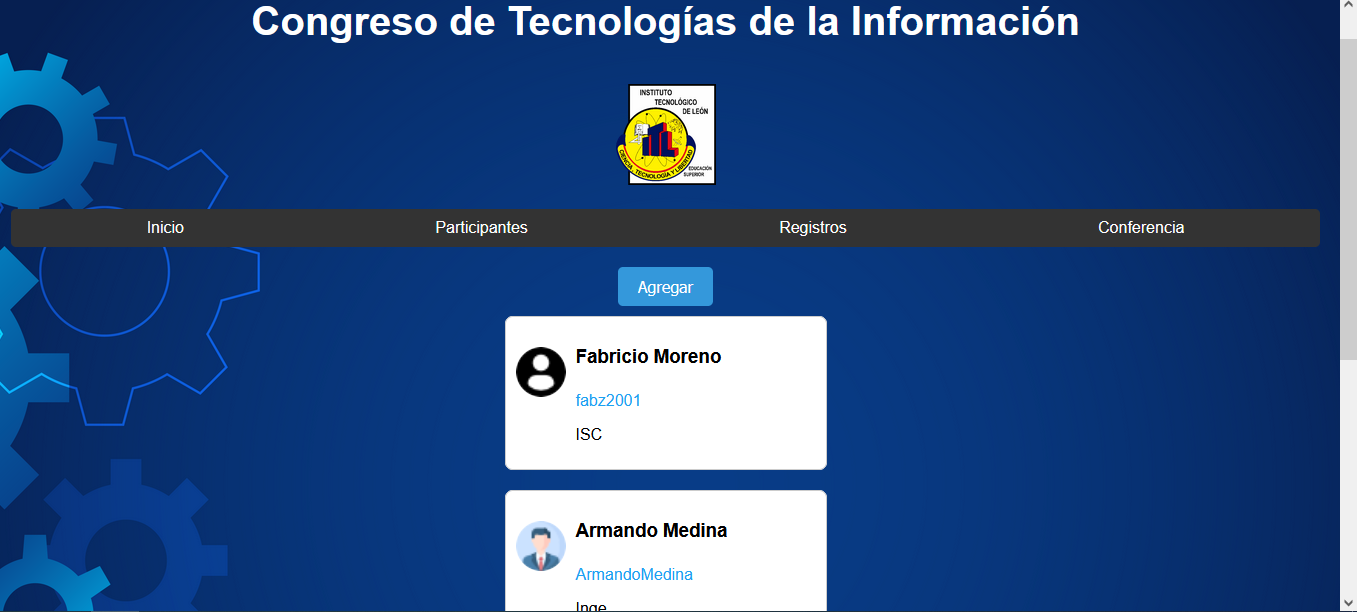
\includegraphics[width=1\linewidth]{Imagenes/web2}
	\caption{Aplicación Web Imagen II}
	\label{fig:web2}
\end{figure}

\begin{figure}[H]
	\centering
	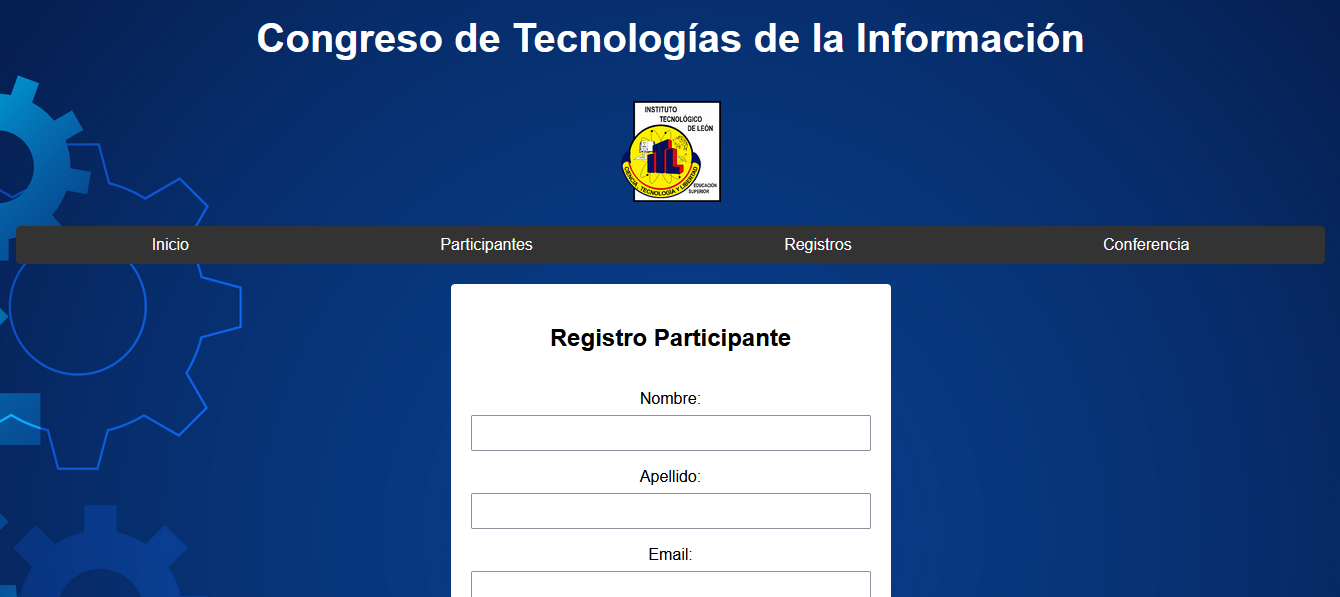
\includegraphics[width=1\linewidth]{Imagenes/web3}
	\caption{Aplicación Web Imagen III}
	\label{fig:web3}
\end{figure}

\begin{figure}[H]
	\centering
	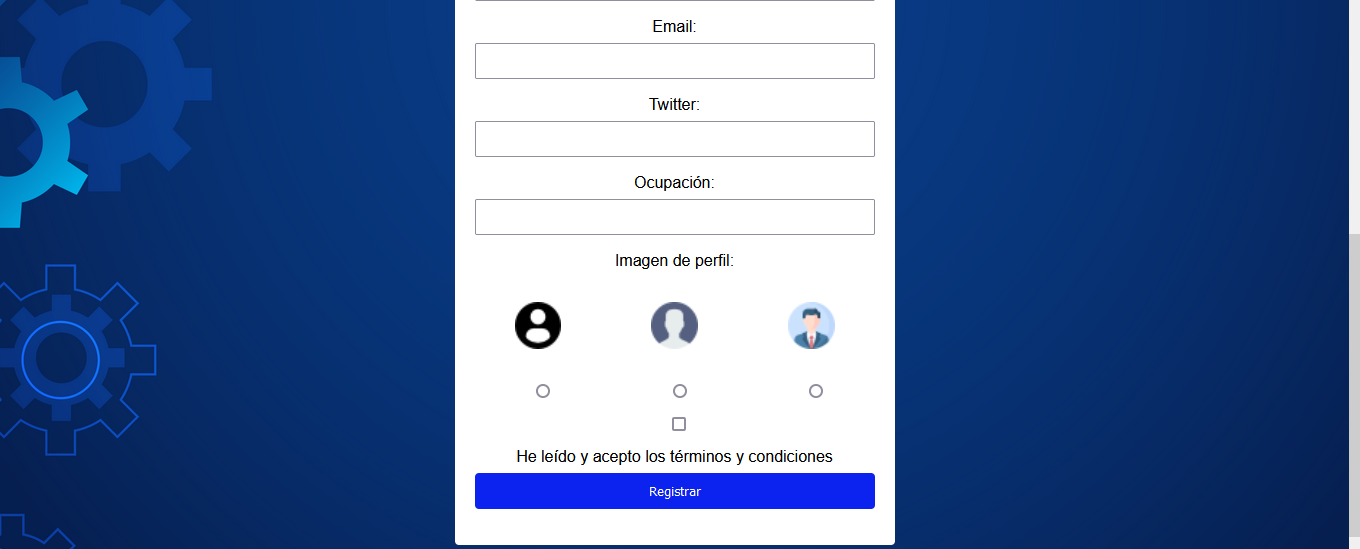
\includegraphics[width=1\linewidth]{Imagenes/web4}
	\caption{Aplicación Web Imagen IV}
	\label{fig:web4}
\end{figure}

\begin{figure}[H]
	\centering
	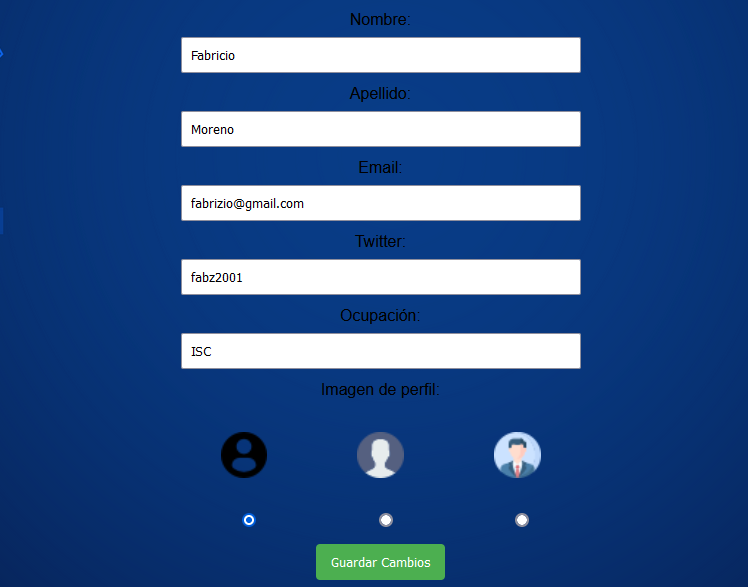
\includegraphics[width=1\linewidth]{Imagenes/web5}
	\caption{Aplicación Web Imagen V}
	\label{fig:web5}
\end{figure}

\begin{figure}[H]
	\centering
	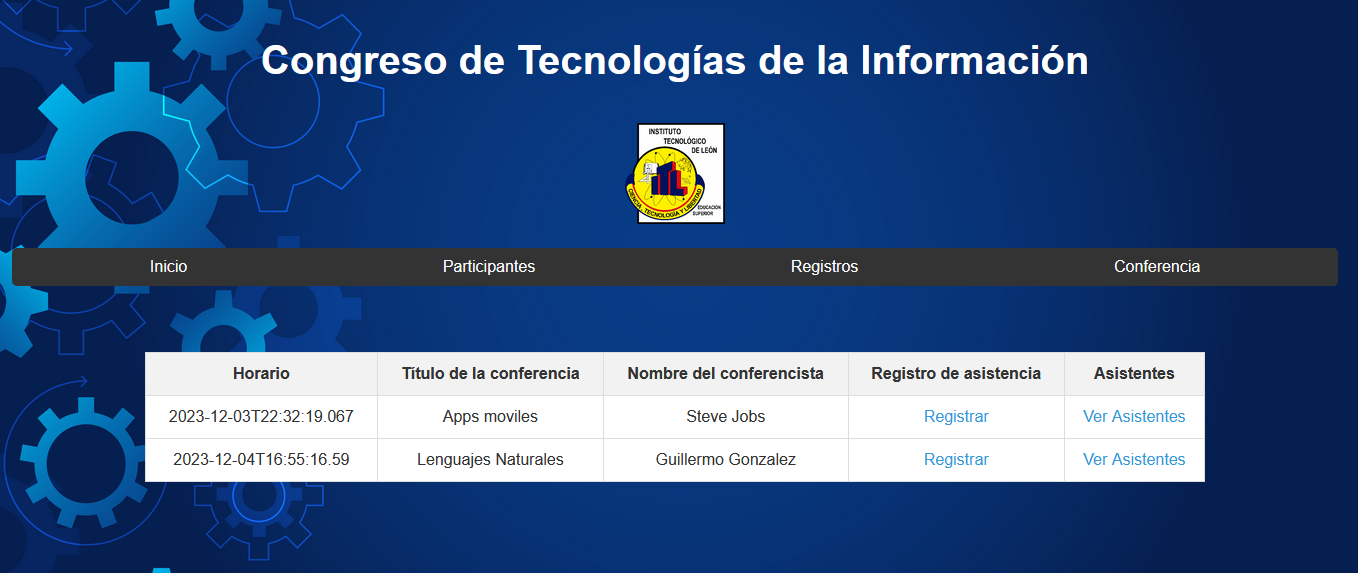
\includegraphics[width=1\linewidth]{Imagenes/web6}
	\caption{Aplicación Web Imagen VI}
	\label{fig:web6}
\end{figure}

\begin{figure}[H]
	\centering
	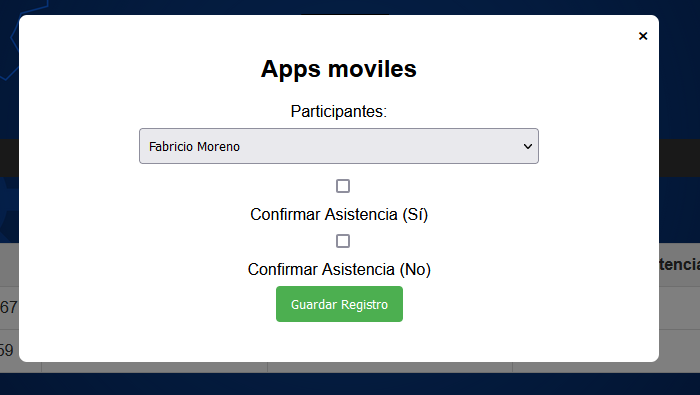
\includegraphics[width=1\linewidth]{Imagenes/web7}
	\caption{Aplicación Web Imagen VII}
	\label{fig:web7}
\end{figure}

\begin{figure}[H]
	\centering
	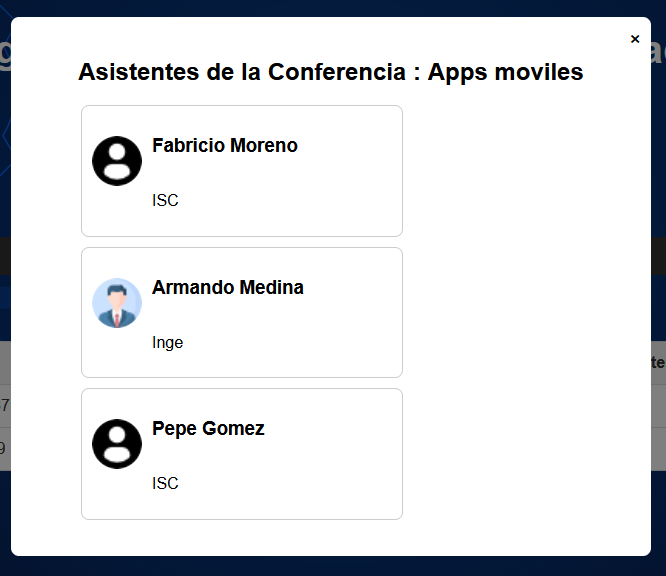
\includegraphics[width=1\linewidth]{Imagenes/web8}
	\caption{Aplicación Web Imagen VIII}
	\label{fig:web8}
\end{figure}

